\documentclass[12pt,letterpaper]{article}
\usepackage[letterpaper,margin=1in]{geometry}

\usepackage{accsupp}
\usepackage{amsmath}
\usepackage{fontspec}
\usepackage{graphicx}
\usepackage{float}
\usepackage{listings,avrlang}
\usepackage{siunitx}
\usepackage{tikz}
\usepackage{xcolor}

% we dont fw ugly
\setmainfont{Palatino ET W02 Roman}[
	BoldFont=Palatino ET W02 Bold,
	ItalicFont=Palatino ET W02 Italic,
	BoldItalicFont=PalatinoETW02-BoldItali,
	Scale=0.8]
\setmonofont{Courier Prime}[Scale=0.9]

% keep page and line numbers from being selected just in awful case
\renewcommand{\thelstnumber}{\protect\BeginAccSupp{ActualText={}}%
	\arabic{lstnumber}%
\protect\EndAccSupp{}}

\renewcommand{\thepage}{\protect\BeginAccSupp{ActualText={}}%
	\arabic{page}%
\protect\EndAccSupp{}}

% for our beautiful schematic
\usetikzlibrary{
	arrows,
	backgrounds,
	calc,
	fit,
	matrix,
	patterns,
	plotmarks,
	shadows,
	shapes,
	snakes
}

\definecolor{Green}{HTML}{006600}
\definecolor{Blue}{HTML}{2d2f92}
\definecolor{Purple}{HTML}{99479b}
\definecolor{Orange}{HTML}{f58137}
\definecolor{Red}{HTML}{ed1b23}
\lstset{
	language=AVR,
	basicstyle=\small\ttfamily,
	keywordstyle=\color{Blue}\bfseries,
	keywordstyle=[2]\color{Orange},
	keywordstyle=[3]\color{Purple},
	keywordstyle=[4]\color{Red},
	commentstyle=\small\itshape\color{Green},
	tabsize=8,
	numbers=left,
	numberstyle=\small\ttfamily\color{Blue}
}

\title{ECE:3360 -- Lab 3 Report}
\author{Oliver Emery and Austin Wittenburg}
\date{9 March 2022}

\begin{document}
\maketitle

\section{Introduction}
The goal of this lab is to get more experience with timers, single-wire 
communication, and rotary pulse generators. We will do this by building a 
thermostat using seven-segment displays, a DHT11 sensor, a rotary pulse 
generator, and a push button switch with a software debounce. The thermostat 
should have two modes. The first mode should allow the user to use the RPG to 
set the desired temperature on the thermostat. The user should know that they 
are in this mode because both of the decimal points on the seven-segment 
displays will be on. When the user pushes the button, the mode should change to 
displaying the actual temperature. Also if the actual temperature is lower than 
the desired temperature, then the yellow LED ``L'' on the Arduino board 
should be turned on, indicating that there is some sort of heating element 
being activated.

\section{Schematic}
Figure 1 shows our circuit design as it was implemented. All resistor values are
\SI{1}{\kilo\ohm}, with the exception of the resistor between the ATmega328P and
the DHT11, which is \SI{330}{\ohm}. The circuit is running on \SI{5}{V}.

\begin{figure}[H]
	\centering
	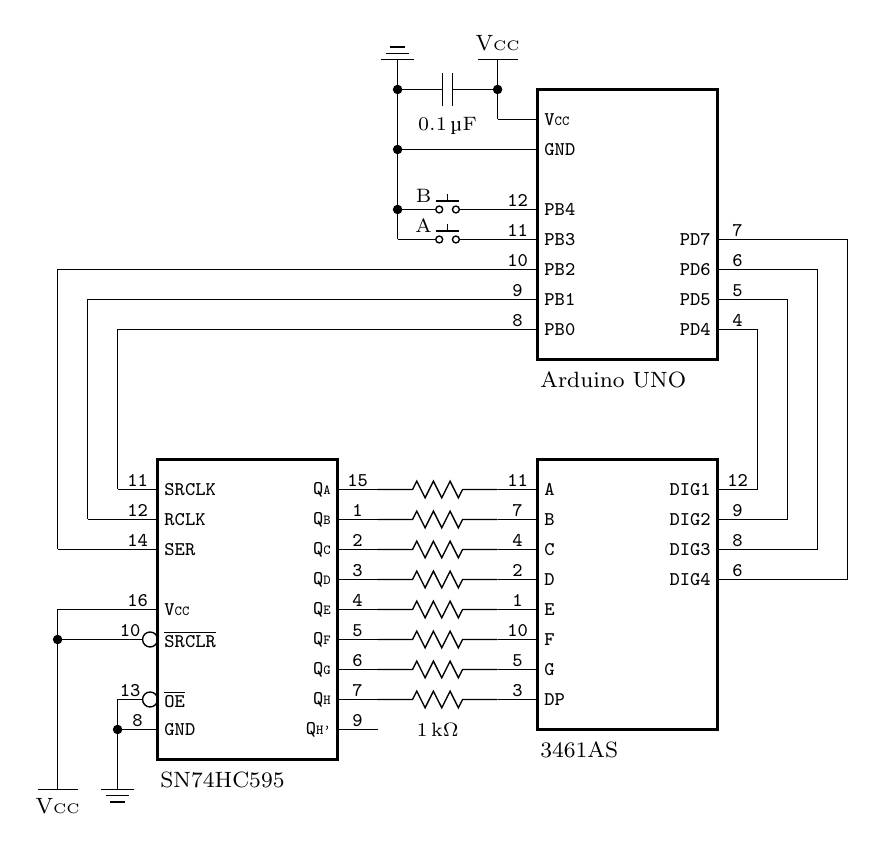
\begin{tikzpicture}[scale=2.54]%
% dpic version 2021.11.01 option -g for TikZ and PGF 1.01
\ifx\dpiclw\undefined\newdimen\dpiclw\fi
\global\def\dpicdraw{\draw[line width=\dpiclw]}
\global\def\dpicstop{;}
\dpiclw=0.8bp
\dpiclw=0.8bp
{\footnotesize
\dpicdraw (0.2,-0.711111) rectangle (1.1,0.788889)\dpicstop
\dpiclw=0.5bp
\draw (0.22,-0.561111) node[right=-2bp]{{\ttfamily\scriptsize GND}};
\dpicdraw (0.2,-0.561111)
 --(-0,-0.561111)\dpicstop
\draw (0.1,-0.561111) node[above=-2bp]{{\ttfamily\scriptsize 8}};
\dpiclw=2bp
\dpiclw=0.5bp
\draw (0.22,-0.411111) node[right=-2bp]{{\ttfamily\scriptsize $\overline{\hbox{OE}}$}};
\dpicdraw (0.1625,-0.411111) circle (0.014764in)\dpicstop
\dpicdraw (0.125,-0.411111)
 --(-0,-0.411111)\dpicstop
\draw (0.0625,-0.411111) node[above=-2bp]{{\ttfamily\scriptsize 13}};
\dpiclw=2bp
\dpiclw=0.5bp
\draw (0.22,-0.111111) node[right=-2bp]{{\ttfamily\scriptsize $\overline{\hbox{SRCLR}}$}};
\dpicdraw (0.1625,-0.111111) circle (0.014764in)\dpicstop
\dpicdraw (0.125,-0.111111)
 --(-0,-0.111111)\dpicstop
\draw (0.0625,-0.111111) node[above=-2bp]{{\ttfamily\scriptsize 10}};
\dpiclw=2bp
\dpiclw=0.5bp
\draw (0.22,0.038889) node[right=-2bp]{{\ttfamily\scriptsize V\hbox{\tiny CC}}};
\dpicdraw (0.2,0.038889)
 --(-0,0.038889)\dpicstop
\draw (0.1,0.038889) node[above=-2bp]{{\ttfamily\scriptsize 16}};
\dpiclw=2bp
\dpiclw=0.5bp
\draw (0.22,0.338889) node[right=-2bp]{{\ttfamily\scriptsize SER}};
\dpicdraw (0.2,0.338889)
 --(-0,0.338889)\dpicstop
\draw (0.1,0.338889) node[above=-2bp]{{\ttfamily\scriptsize 14}};
\dpiclw=2bp
\dpiclw=0.5bp
\draw (0.22,0.488889) node[right=-2bp]{{\ttfamily\scriptsize RCLK}};
\dpicdraw (0.2,0.488889)
 --(-0,0.488889)\dpicstop
\draw (0.1,0.488889) node[above=-2bp]{{\ttfamily\scriptsize 12}};
\dpiclw=2bp
\dpiclw=0.5bp
\draw (0.22,0.638889) node[right=-2bp]{{\ttfamily\scriptsize SRCLK}};
\dpicdraw (0.2,0.638889)
 --(-0,0.638889)\dpicstop
\draw (0.1,0.638889) node[above=-2bp]{{\ttfamily\scriptsize 11}};
\dpiclw=2bp
\dpiclw=0.5bp
\draw (1.08,-0.561111) node[left=-2bp]{{\ttfamily\scriptsize Q\hbox{\tiny H\rq}}};
\dpicdraw (1.1,-0.561111)
 --(1.3,-0.561111)\dpicstop
\draw (1.2,-0.561111) node[above=-2bp]{{\ttfamily\scriptsize 9}};
\dpiclw=2bp
\dpiclw=0.5bp
\draw (1.08,-0.411111) node[left=-2bp]{{\ttfamily\scriptsize Q\hbox{\tiny H}}};
\dpicdraw (1.1,-0.411111)
 --(1.3,-0.411111)\dpicstop
\draw (1.2,-0.411111) node[above=-2bp]{{\ttfamily\scriptsize 7}};
\dpiclw=2bp
\dpiclw=0.5bp
\draw (1.08,-0.261111) node[left=-2bp]{{\ttfamily\scriptsize Q\hbox{\tiny G}}};
\dpicdraw (1.1,-0.261111)
 --(1.3,-0.261111)\dpicstop
\draw (1.2,-0.261111) node[above=-2bp]{{\ttfamily\scriptsize 6}};
\dpiclw=2bp
\dpiclw=0.5bp
\draw (1.08,-0.111111) node[left=-2bp]{{\ttfamily\scriptsize Q\hbox{\tiny F}}};
\dpicdraw (1.1,-0.111111)
 --(1.3,-0.111111)\dpicstop
\draw (1.2,-0.111111) node[above=-2bp]{{\ttfamily\scriptsize 5}};
\dpiclw=2bp
\dpiclw=0.5bp
\draw (1.08,0.038889) node[left=-2bp]{{\ttfamily\scriptsize Q\hbox{\tiny E}}};
\dpicdraw (1.1,0.038889)
 --(1.3,0.038889)\dpicstop
\draw (1.2,0.038889) node[above=-2bp]{{\ttfamily\scriptsize 4}};
\dpiclw=2bp
\dpiclw=0.5bp
\draw (1.08,0.188889) node[left=-2bp]{{\ttfamily\scriptsize Q\hbox{\tiny D}}};
\dpicdraw (1.1,0.188889)
 --(1.3,0.188889)\dpicstop
\draw (1.2,0.188889) node[above=-2bp]{{\ttfamily\scriptsize 3}};
\dpiclw=2bp
\dpiclw=0.5bp
\draw (1.08,0.338889) node[left=-2bp]{{\ttfamily\scriptsize Q\hbox{\tiny C}}};
\dpicdraw (1.1,0.338889)
 --(1.3,0.338889)\dpicstop
\draw (1.2,0.338889) node[above=-2bp]{{\ttfamily\scriptsize 2}};
\dpiclw=2bp
\dpiclw=0.5bp
\draw (1.08,0.488889) node[left=-2bp]{{\ttfamily\scriptsize Q\hbox{\tiny B}}};
\dpicdraw (1.1,0.488889)
 --(1.3,0.488889)\dpicstop
\draw (1.2,0.488889) node[above=-2bp]{{\ttfamily\scriptsize 1}};
\dpiclw=2bp
\dpiclw=0.5bp
\draw (1.08,0.638889) node[left=-2bp]{{\ttfamily\scriptsize Q\hbox{\tiny A}}};
\dpicdraw (1.1,0.638889)
 --(1.3,0.638889)\dpicstop
\draw (1.2,0.638889) node[above=-2bp]{{\ttfamily\scriptsize 15}};
\dpiclw=2bp
\draw (0.2,-0.761111) node[below right=-2bp]{SN74HC595};
\dpiclw=0.8bp
\dpicdraw (2.1,-0.561111) rectangle (3,0.788889)\dpicstop
\dpiclw=0.5bp
\draw (2.12,-0.411111) node[right=-2bp]{{\ttfamily\scriptsize DP}};
\dpicdraw (2.1,-0.411111)
 --(1.9,-0.411111)\dpicstop
\draw (2,-0.411111) node[above=-2bp]{{\ttfamily\scriptsize 3}};
\dpiclw=2bp
\dpiclw=0.5bp
\draw (2.12,-0.261111) node[right=-2bp]{{\ttfamily\scriptsize G}};
\dpicdraw (2.1,-0.261111)
 --(1.9,-0.261111)\dpicstop
\draw (2,-0.261111) node[above=-2bp]{{\ttfamily\scriptsize 5}};
\dpiclw=2bp
\dpiclw=0.5bp
\draw (2.12,-0.111111) node[right=-2bp]{{\ttfamily\scriptsize F}};
\dpicdraw (2.1,-0.111111)
 --(1.9,-0.111111)\dpicstop
\draw (2,-0.111111) node[above=-2bp]{{\ttfamily\scriptsize 10}};
\dpiclw=2bp
\dpiclw=0.5bp
\draw (2.12,0.038889) node[right=-2bp]{{\ttfamily\scriptsize E}};
\dpicdraw (2.1,0.038889)
 --(1.9,0.038889)\dpicstop
\draw (2,0.038889) node[above=-2bp]{{\ttfamily\scriptsize 1}};
\dpiclw=2bp
\dpiclw=0.5bp
\draw (2.12,0.188889) node[right=-2bp]{{\ttfamily\scriptsize D}};
\dpicdraw (2.1,0.188889)
 --(1.9,0.188889)\dpicstop
\draw (2,0.188889) node[above=-2bp]{{\ttfamily\scriptsize 2}};
\dpiclw=2bp
\dpiclw=0.5bp
\draw (2.12,0.338889) node[right=-2bp]{{\ttfamily\scriptsize C}};
\dpicdraw (2.1,0.338889)
 --(1.9,0.338889)\dpicstop
\draw (2,0.338889) node[above=-2bp]{{\ttfamily\scriptsize 4}};
\dpiclw=2bp
\dpiclw=0.5bp
\draw (2.12,0.488889) node[right=-2bp]{{\ttfamily\scriptsize B}};
\dpicdraw (2.1,0.488889)
 --(1.9,0.488889)\dpicstop
\draw (2,0.488889) node[above=-2bp]{{\ttfamily\scriptsize 7}};
\dpiclw=2bp
\dpiclw=0.5bp
\draw (2.12,0.638889) node[right=-2bp]{{\ttfamily\scriptsize A}};
\dpicdraw (2.1,0.638889)
 --(1.9,0.638889)\dpicstop
\draw (2,0.638889) node[above=-2bp]{{\ttfamily\scriptsize 11}};
\dpiclw=2bp
\dpiclw=0.5bp
\draw (2.98,0.188889) node[left=-2bp]{{\ttfamily\scriptsize DIG4}};
\dpicdraw (3,0.188889)
 --(3.2,0.188889)\dpicstop
\draw (3.1,0.188889) node[above=-2bp]{{\ttfamily\scriptsize 6}};
\dpiclw=2bp
\dpiclw=0.5bp
\draw (2.98,0.338889) node[left=-2bp]{{\ttfamily\scriptsize DIG3}};
\dpicdraw (3,0.338889)
 --(3.2,0.338889)\dpicstop
\draw (3.1,0.338889) node[above=-2bp]{{\ttfamily\scriptsize 8}};
\dpiclw=2bp
\dpiclw=0.5bp
\draw (2.98,0.488889) node[left=-2bp]{{\ttfamily\scriptsize DIG2}};
\dpicdraw (3,0.488889)
 --(3.2,0.488889)\dpicstop
\draw (3.1,0.488889) node[above=-2bp]{{\ttfamily\scriptsize 9}};
\dpiclw=2bp
\dpiclw=0.5bp
\draw (2.98,0.638889) node[left=-2bp]{{\ttfamily\scriptsize DIG1}};
\dpicdraw (3,0.638889)
 --(3.2,0.638889)\dpicstop
\draw (3.1,0.638889) node[above=-2bp]{{\ttfamily\scriptsize 12}};
\dpiclw=2bp
\draw (2.1,-0.611111) node[below right=-2bp]{3461AS};
\dpiclw=0.8bp
\dpicdraw (2.1,1.288889) rectangle (3,2.638889)\dpicstop
\dpiclw=0.5bp
\draw (2.12,1.438889) node[right=-2bp]{{\ttfamily\scriptsize PB0}};
\dpicdraw (2.1,1.438889)
 --(1.9,1.438889)\dpicstop
\draw (2,1.438889) node[above=-2bp]{{\ttfamily\scriptsize 8}};
\dpiclw=2bp
\dpiclw=0.5bp
\draw (2.12,1.588889) node[right=-2bp]{{\ttfamily\scriptsize PB1}};
\dpicdraw (2.1,1.588889)
 --(1.9,1.588889)\dpicstop
\draw (2,1.588889) node[above=-2bp]{{\ttfamily\scriptsize 9}};
\dpiclw=2bp
\dpiclw=0.5bp
\draw (2.12,1.738889) node[right=-2bp]{{\ttfamily\scriptsize PB2}};
\dpicdraw (2.1,1.738889)
 --(1.9,1.738889)\dpicstop
\draw (2,1.738889) node[above=-2bp]{{\ttfamily\scriptsize 10}};
\dpiclw=2bp
\dpiclw=0.5bp
\draw (2.12,1.888889) node[right=-2bp]{{\ttfamily\scriptsize PB3}};
\dpicdraw (2.1,1.888889)
 --(1.9,1.888889)\dpicstop
\draw (2,1.888889) node[above=-2bp]{{\ttfamily\scriptsize 11}};
\dpiclw=2bp
\dpiclw=0.5bp
\draw (2.12,2.038889) node[right=-2bp]{{\ttfamily\scriptsize PB4}};
\dpicdraw (2.1,2.038889)
 --(1.9,2.038889)\dpicstop
\draw (2,2.038889) node[above=-2bp]{{\ttfamily\scriptsize 12}};
\dpiclw=2bp
\dpiclw=0.5bp
\draw (2.12,2.338889) node[right=-2bp]{{\ttfamily\scriptsize GND}};
\dpicdraw (2.1,2.338889)
 --(1.9,2.338889)\dpicstop
\dpiclw=2bp
\dpiclw=0.5bp
\draw (2.12,2.488889) node[right=-2bp]{{\ttfamily\scriptsize V\hbox{\tiny CC}}};
\dpicdraw (2.1,2.488889)
 --(1.9,2.488889)\dpicstop
\dpiclw=2bp
\dpiclw=0.5bp
\draw (2.98,1.438889) node[left=-2bp]{{\ttfamily\scriptsize PD4}};
\dpicdraw (3,1.438889)
 --(3.2,1.438889)\dpicstop
\draw (3.1,1.438889) node[above=-2bp]{{\ttfamily\scriptsize 4}};
\dpiclw=2bp
\dpiclw=0.5bp
\draw (2.98,1.588889) node[left=-2bp]{{\ttfamily\scriptsize PD5}};
\dpicdraw (3,1.588889)
 --(3.2,1.588889)\dpicstop
\draw (3.1,1.588889) node[above=-2bp]{{\ttfamily\scriptsize 5}};
\dpiclw=2bp
\dpiclw=0.5bp
\draw (2.98,1.738889) node[left=-2bp]{{\ttfamily\scriptsize PD6}};
\dpicdraw (3,1.738889)
 --(3.2,1.738889)\dpicstop
\draw (3.1,1.738889) node[above=-2bp]{{\ttfamily\scriptsize 6}};
\dpiclw=2bp
\dpiclw=0.5bp
\draw (2.98,1.888889) node[left=-2bp]{{\ttfamily\scriptsize PD7}};
\dpicdraw (3,1.888889)
 --(3.2,1.888889)\dpicstop
\draw (3.1,1.888889) node[above=-2bp]{{\ttfamily\scriptsize 7}};
\dpiclw=2bp
\draw (2.1,1.238889) node[below right=-2bp]{Arduino UNO};
\dpiclw=0.8bp
\dpiclw=0.5bp
\dpicdraw (1.3,0.638889)
 --(1.475,0.638889)
 --(1.495833,0.680556)
 --(1.5375,0.597222)
 --(1.579167,0.680556)
 --(1.620833,0.597222)
 --(1.6625,0.680556)
 --(1.704167,0.597222)
 --(1.725,0.638889)
 --(1.9,0.638889)\dpicstop
\dpicdraw (1.3,0.488889)
 --(1.475,0.488889)
 --(1.495833,0.530556)
 --(1.5375,0.447222)
 --(1.579167,0.530556)
 --(1.620833,0.447222)
 --(1.6625,0.530556)
 --(1.704167,0.447222)
 --(1.725,0.488889)
 --(1.9,0.488889)\dpicstop
\dpicdraw (1.3,0.338889)
 --(1.475,0.338889)
 --(1.495833,0.380556)
 --(1.5375,0.297222)
 --(1.579167,0.380556)
 --(1.620833,0.297222)
 --(1.6625,0.380556)
 --(1.704167,0.297222)
 --(1.725,0.338889)
 --(1.9,0.338889)\dpicstop
\dpicdraw (1.3,0.188889)
 --(1.475,0.188889)
 --(1.495833,0.230556)
 --(1.5375,0.147222)
 --(1.579167,0.230556)
 --(1.620833,0.147222)
 --(1.6625,0.230556)
 --(1.704167,0.147222)
 --(1.725,0.188889)
 --(1.9,0.188889)\dpicstop
\dpicdraw (1.3,0.038889)
 --(1.475,0.038889)
 --(1.495833,0.080556)
 --(1.5375,-0.002778)
 --(1.579167,0.080556)
 --(1.620833,-0.002778)
 --(1.6625,0.080556)
 --(1.704167,-0.002778)
 --(1.725,0.038889)
 --(1.9,0.038889)\dpicstop
\dpicdraw (1.3,-0.111111)
 --(1.475,-0.111111)
 --(1.495833,-0.069444)
 --(1.5375,-0.152778)
 --(1.579167,-0.069444)
 --(1.620833,-0.152778)
 --(1.6625,-0.069444)
 --(1.704167,-0.152778)
 --(1.725,-0.111111)
 --(1.9,-0.111111)\dpicstop
\dpicdraw (1.3,-0.261111)
 --(1.475,-0.261111)
 --(1.495833,-0.219444)
 --(1.5375,-0.302778)
 --(1.579167,-0.219444)
 --(1.620833,-0.302778)
 --(1.6625,-0.219444)
 --(1.704167,-0.302778)
 --(1.725,-0.261111)
 --(1.9,-0.261111)\dpicstop
\dpicdraw (1.3,-0.411111)
 --(1.475,-0.411111)
 --(1.495833,-0.369444)
 --(1.5375,-0.452778)
 --(1.579167,-0.369444)
 --(1.620833,-0.452778)
 --(1.6625,-0.369444)
 --(1.704167,-0.452778)
 --(1.725,-0.411111)
 --(1.9,-0.411111)\dpicstop
\draw (1.6,-0.561111) node{\scriptsize \SI{1}{\kilo\ohm}};
\dpicdraw (0,-0.411111)
 --(0,-0.861111)\dpicstop
\dpicdraw (0.083333,-0.861111)
 --(-0.083333,-0.861111)\dpicstop
\dpicdraw (0.055556,-0.892361)
 --(-0.055556,-0.892361)\dpicstop
\dpicdraw (0.035714,-0.923611)
 --(-0.035714,-0.923611)\dpicstop
\dpicdraw[fill=black](-0,-0.561111) circle (0.007874in)\dpicstop
\dpicdraw (3.2,1.438889)
 --(3.2,0.638889)\dpicstop
\dpicdraw (3.2,1.588889)
 --(3.35,1.588889)\dpicstop
\dpicdraw (3.35,1.588889)
 --(3.35,0.488889)\dpicstop
\dpicdraw (3.35,0.488889)
 --(3.2,0.488889)\dpicstop
\dpicdraw (3.2,1.738889)
 --(3.5,1.738889)\dpicstop
\dpicdraw (3.5,1.738889)
 --(3.5,0.338889)\dpicstop
\dpicdraw (3.5,0.338889)
 --(3.2,0.338889)\dpicstop
\dpicdraw (3.2,1.888889)
 --(3.65,1.888889)\dpicstop
\dpicdraw (3.65,1.888889)
 --(3.65,0.188889)\dpicstop
\dpicdraw (3.65,0.188889)
 --(3.2,0.188889)\dpicstop
\dpicdraw (1.9,1.438889)
 --(0,1.438889)\dpicstop
\dpicdraw (0,1.438889)
 --(-0,0.638889)\dpicstop
\dpicdraw (1.9,1.588889)
 --(-0.15,1.588889)\dpicstop
\dpicdraw (-0.15,1.588889)
 --(-0.15,0.488889)\dpicstop
\dpicdraw (-0.15,0.488889)
 --(-0,0.488889)\dpicstop
\dpicdraw (1.9,1.738889)
 --(-0.3,1.738889)\dpicstop
\dpicdraw (-0.3,1.738889)
 --(-0.3,0.338889)\dpicstop
\dpicdraw (-0.3,0.338889)
 --(-0,0.338889)\dpicstop
\dpicdraw (1.4,1.888889)
 --(1.591037,1.888889)\dpicstop
\dpicdraw (1.608333,1.888889) circle (0.00681in)\dpicstop
\dpicdraw (1.691667,1.888889) circle (0.00681in)\dpicstop
\dpicdraw (1.591037,1.93213)
 --(1.708963,1.93213)\dpicstop
\dpicdraw (1.65,1.93213)
 --(1.65,1.966723)\dpicstop
\dpicdraw (1.708963,1.888889)
 --(1.9,1.888889)\dpicstop
\dpicdraw (1.4,2.038889)
 --(1.591037,2.038889)\dpicstop
\dpicdraw (1.608333,2.038889) circle (0.00681in)\dpicstop
\dpicdraw (1.691667,2.038889) circle (0.00681in)\dpicstop
\dpicdraw (1.591037,2.08213)
 --(1.708963,2.08213)\dpicstop
\dpicdraw (1.65,2.08213)
 --(1.65,2.116723)\dpicstop
\dpicdraw (1.708963,2.038889)
 --(1.9,2.038889)\dpicstop
\dpicdraw (1.9,2.338889)
 --(1.4,2.338889)\dpicstop
\dpicdraw (1.4,1.888889)
 --(1.4,2.788889)\dpicstop
\dpicdraw (1.316667,2.788889)
 --(1.483333,2.788889)\dpicstop
\dpicdraw (1.344444,2.820139)
 --(1.455556,2.820139)\dpicstop
\dpicdraw (1.364286,2.851389)
 --(1.435714,2.851389)\dpicstop
\dpicdraw[fill=black](1.4,2.038889) circle (0.007874in)\dpicstop
\dpicdraw[fill=black](1.4,2.338889) circle (0.007874in)\dpicstop
\dpicdraw (1.9,2.488889)
 --(1.9,2.788889)\dpicstop
\draw (1.9,2.818889) node[above=-2bp]{V\hbox{\tiny CC}};
\dpicdraw (1.8,2.788889)
 --(2,2.788889)\dpicstop
\dpicdraw (1.4,2.638889)
 --(1.625,2.638889)\dpicstop
\dpicdraw (1.625,2.555556)
 --(1.625,2.722222)\dpicstop
\dpicdraw (1.675,2.555556)
 --(1.675,2.722222)\dpicstop
\dpicdraw (1.675,2.638889)
 --(1.9,2.638889)\dpicstop
\draw (1.65,2.458889) node{\scriptsize\SI{0.1}{\micro\farad}};
\dpicdraw[fill=black](1.4,2.638889) circle (0.007874in)\dpicstop
\dpicdraw[fill=black](1.9,2.638889) circle (0.007874in)\dpicstop
\dpicdraw (0,-0.111111)
 --(-0.3,-0.111111)\dpicstop
\dpicdraw (-0,0.038889)
 --(-0.3,0.038889)\dpicstop
\dpicdraw (-0.3,0.038889)
 --(-0.3,-0.861111)\dpicstop
\draw (-0.3,-0.891111) node[below=-2bp]{V\hbox{\tiny CC}};
\dpicdraw (-0.4,-0.861111)
 --(-0.2,-0.861111)\dpicstop
\dpicdraw[fill=black](-0.3,-0.111111) circle (0.007874in)\dpicstop
\draw (1.53,2.108889) node{{\scriptsize B}};
\draw (1.53,1.958889) node{{\scriptsize A}};
}
\end{tikzpicture}%

	\caption{schematic as implemented}
\end{figure}
\begin{figure}[H]
	\centering
	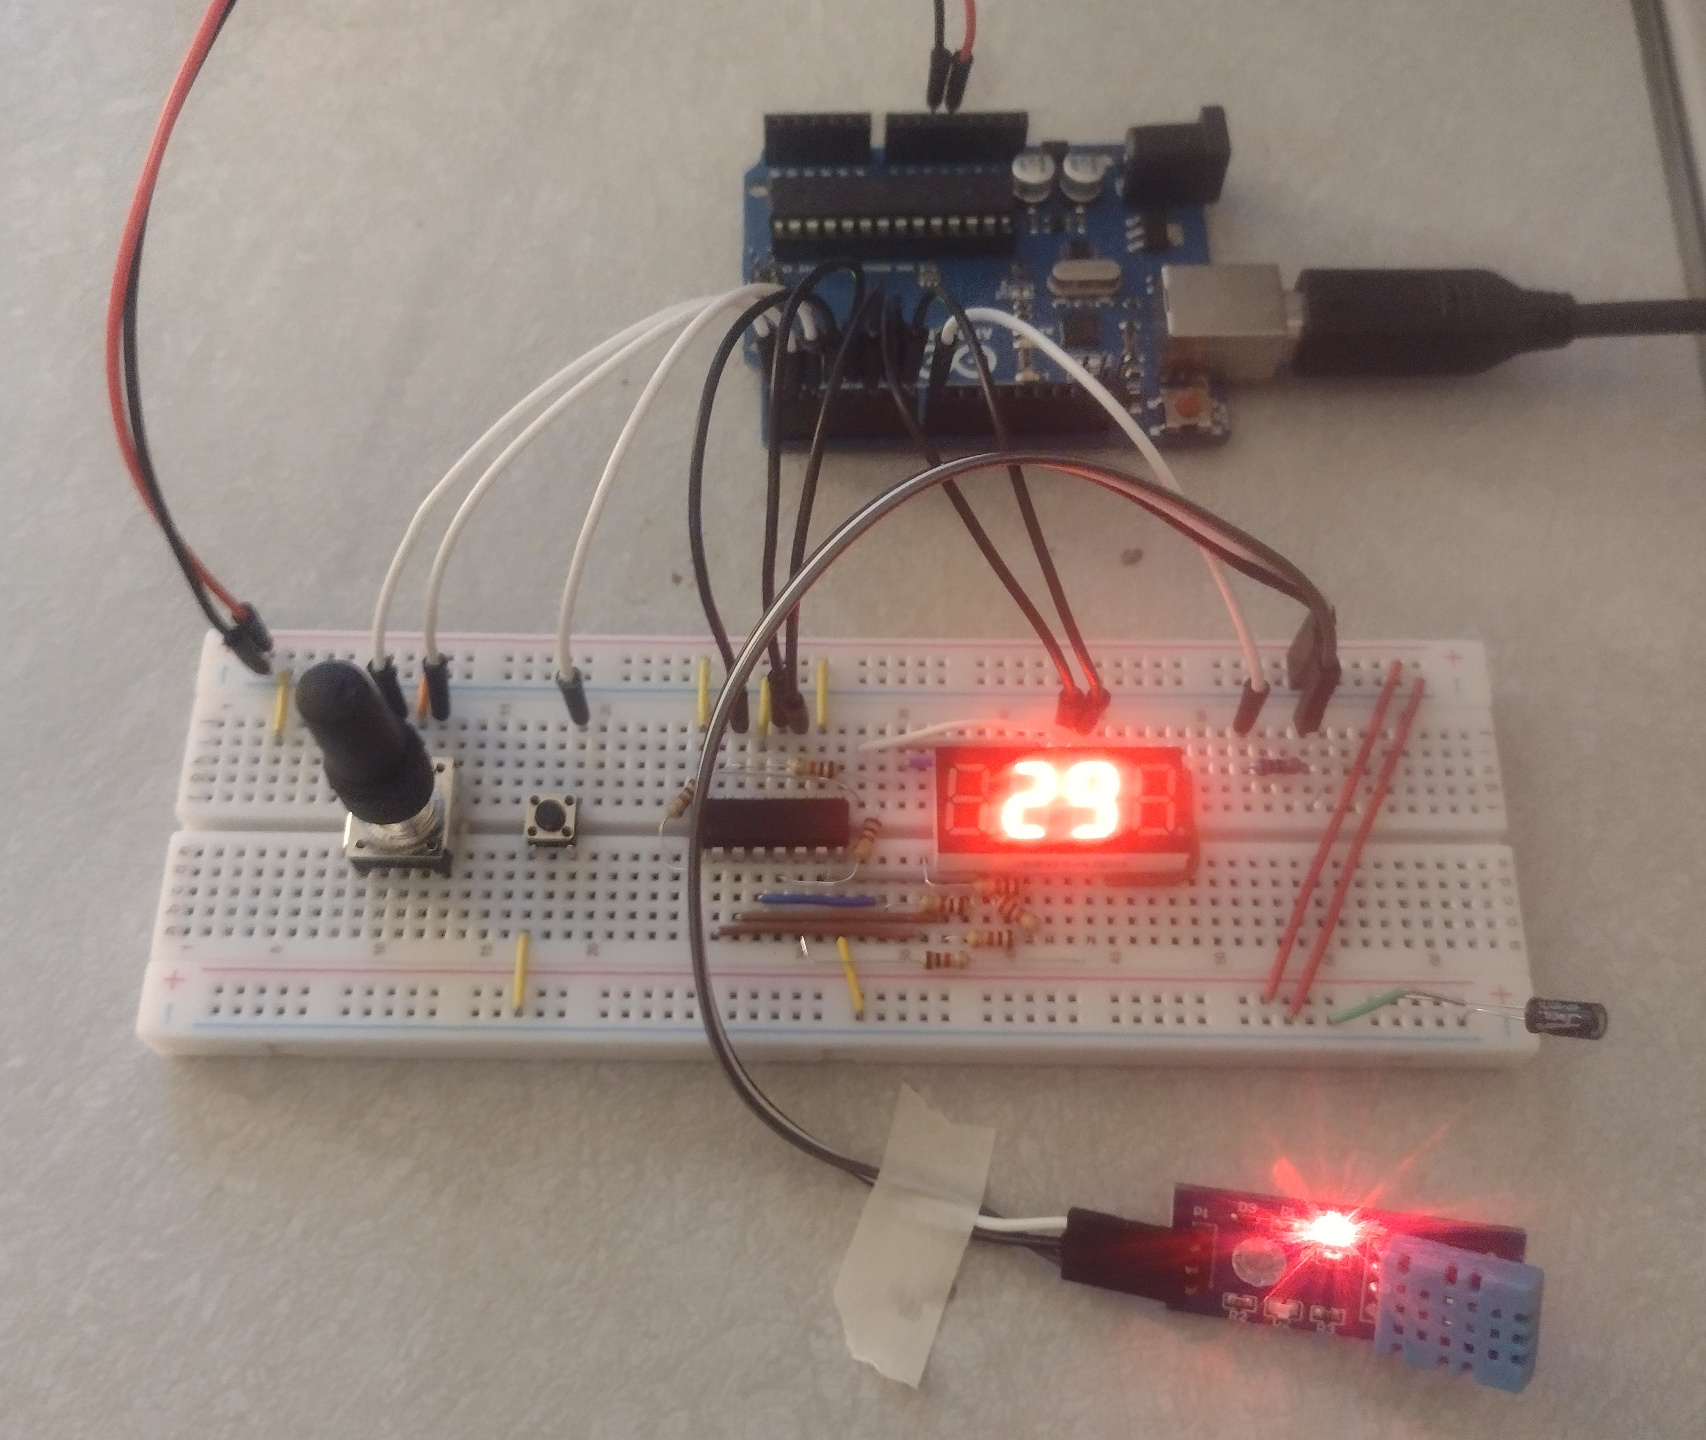
\includegraphics[width=0.7\textwidth]{breadboard.jpg}
	\caption{physical implementation}
\end{figure}

\section{Discussion}
The software debounce we used in this lab is similar to the debounce method we 
used in lab 2, but we essentially just treated the RPG as two buttons when we 
were debouncing it. In fact a lot of our setup was carried over from lab 2 
including the placement and wiring of the shift register and seven-segment 
display. Using the serial connection to communicate with the DHT11 was trickier 
than expected. We ran into a lot of problems with timing the signal to be able 
to read it reliably every time.

\subsection*{Timer Usage}
We used one 8-bit timer for all time-based operations. For the majority of each
second during which the DHT11 is not being read, we have the timer configured in
clear timer on compare match mode. The compare register is set to target a \SI{250}{\micro\second}
interval between compare match flags.
\par\vspace*{2ex}
While reading the DHT11, we use a /8 prescaler for \SI{0.5}{\micro\second} resolution,
and compare-timer-on-match mode as well.

\subsection*{Reading the DHT11}
As an aid in designing the sensor data reading subroutine, we pulled a transaction sample
from an oscilloscope and loaded it into PulseView, a frontend for \texttt{sigrok}. We wrote
a protocol decoder for DHT11 messages to gain a better understanding of the signal format.
\begin{figure}[H]
	\centering
	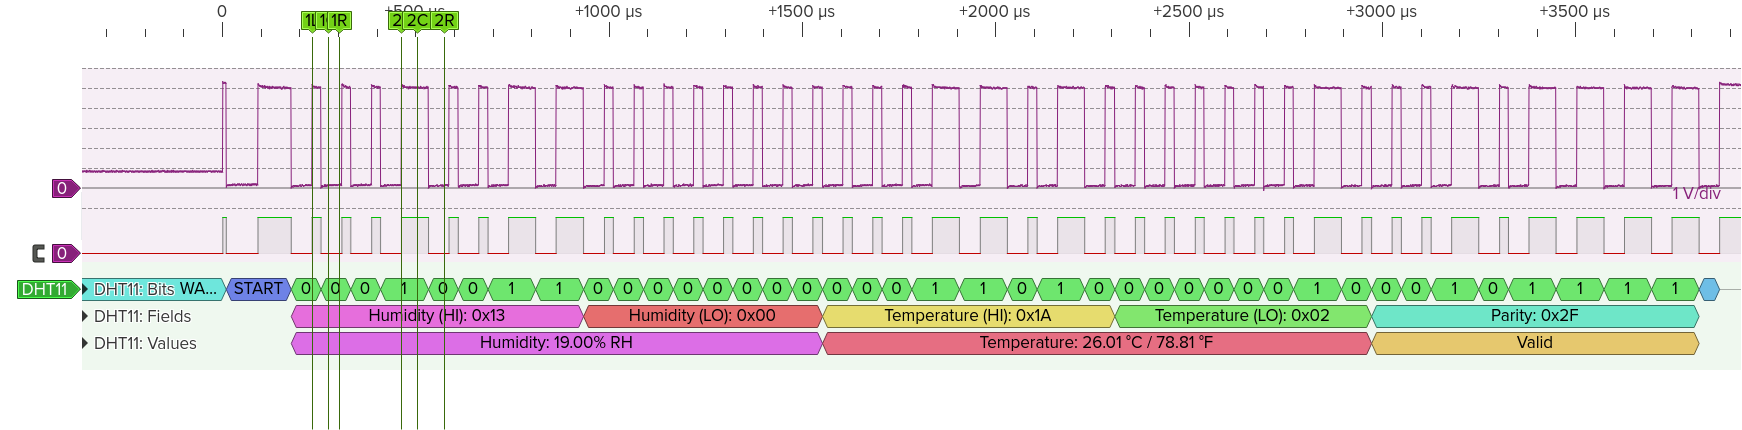
\includegraphics[width=\linewidth]{sigrok-pulseview.png}
	\caption{PulseView display with custom protocol decoder}
\end{figure}
Our timing algorithm is illustrated in Figure 4. We first synchronize to the positive clock
edge of the current bit (1L, 2L), then delay for \SI{40}{\micro\second}. At this time, the
subroutine reads the sensor data pin value (1C, 2C). If the pin is lo (1C), this indicates a
0, and vice versa. Finally, we wait for the next positive clock edge.
\begin{figure}[H]
	\centering
	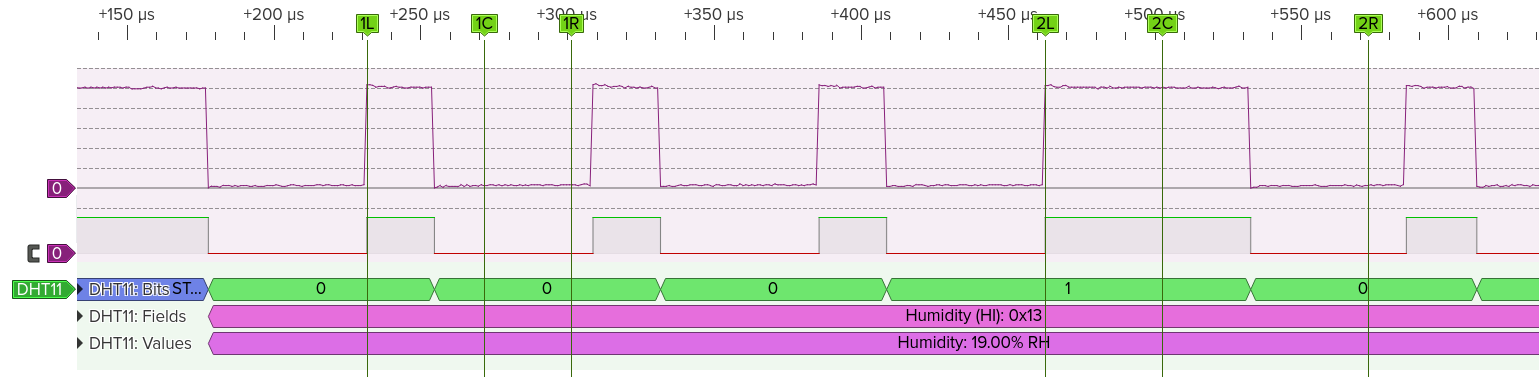
\includegraphics[width=\linewidth]{reading-dht11.png}
	\caption{sensor read subroutine intervals}
\end{figure}



\section{Conclusion}
This lab helped us better understand the serial communications through the 
DHT11, and gave us much more experience with using timers. We were able to 
implement the RPG very easily by treating it similar to just two buttons which 
allowed us to reuse our previous methods for debouncing which were already very 
effective.

\newpage\appendix
\section{Source Code Listing}
\lstinputlisting{../main.S}

\section{References}
\begin{enumerate}
	\item ``DHT11 Datasheet'' <https://www.mouser.com/datasheet/2/758/DHT11-Technical-Data-Sheet-Translated-Version-1143054.pdf>
	\item ``SN74HC595 Datasheet'' <https://www.sparkfun.com/datasheets/IC/SN74HC595.pdf>
	\item ``3461AS Datasheet'' <http://www.xlitx.com/datasheet/3461AS.pdf>
\end{enumerate}
\end{document}
